\documentclass{article}

\usepackage{geometry}
\usepackage{multicol}
\usepackage{fixltx2e}


\usepackage{Sweave}
\begin{document}
\Sconcordance{concordance:rainFallReport.tex:rainFallReport.Rnw:%
1 7 1 1 0 2 1 1 4 36 1 1 24 1 3 6 1 1 5 4 0 1 1 1 3 1 0 1 1 1 3 1 0 2 1 %
1 2 1 11 10 0 1 2 2 1 1 2 4 0 1 3 2 1 1 6 5 0 1 1 1 5 3 0 1 1 1 5 3 0 1 %
4 3 0 1 2 1 4 3 0 1 12 9 0 1 9 7 0 1 6 4 0 1 1 1 9 7 0 1 2 1 5 3 0 1 6 %
3 0 1 1 1 4 2 0 1 8 6 0 1 3 2 0 1 2 1 0 1 3 1 0 1 3 2 0 2 2 1 0 1 2 1 0 %
1 5 3 0 2 2 5 0 1 3}



\newgeometry{margin=3cm}

\begin{center}
\begin{huge}
Mosquito population and rainfall: summer 2013 \\
\end{huge}

\begin{small}
Joe Brew
\end{small}

\end{center}

\begin{multicols}{2}
\subsection*{Question}
Which rainfall period best predicted mosquito population for summer 2013?\\

\subsection*{Methods}
Daily rainfall data for all of 2013 was "webscraped" from wunderground.com (see webscraping code in appendix).  \\

Mosquito trap data was provided by Clark Scientific and compiled by ACHD. \\

A simulation model was run to determine the highest possible R-squared between:\\

\noindent Y = Number of mosquitoes trapped on date Z \\
\noindent X = Cumulative rainfall for range Z\textsubscript{range}\\
\noindent Z\textsubscript{range} = Z-A and Z-B. The limits for A and B were set at 5 and 20. \\

The simulation compared 264 unique prediction possibilites for all the unique iterations of Z\textsubscript{range}. \\

\subsection*{Results}
The association between Z\textsubscript{range} and Y was strongest (R-squared = 0.164) for the range from 17-27 days prior to trap collection. In other words, mosquito population is predicted to surge in the period 17-27 days following a heavy rain.  

\end{multicols}
\begin{center}
\setkeys{Gin}{width=1.1\textwidth}
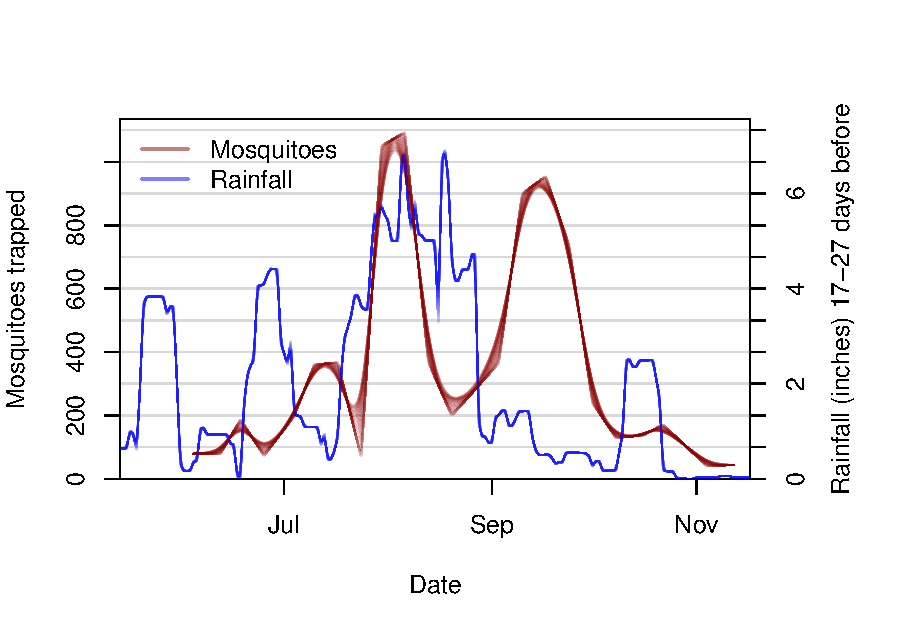
\includegraphics{rainFallReport-002}
\end{center}

\newpage
\section*{Appendix}

\subsection*{Webscraping code}

\begin{Schunk}
\begin{Sinput}
> #THE FOLLOWING SCRIPT TAKES RAINFALL DATA FROM WUNDERGROUND
> 
> #Establish start and end dates
> startDate <- "2013-03-01"
> nDays <- 270
> #Set up URL
> linkPart1 <- "http://www.wunderground.com/history/airport/KGNV/"
> linkPart3 <-  "/DailyHistory.html"
> ts <- as.data.frame(c(as.Date(startDate, format="%Y-%m-%d"), 
+                       as.Date(startDate, format="%Y-%m-%d")+1:(nDays-1)))
> colnames(ts) <- "date"
> ts$dateRec <- format(ts$date, format="%Y/%m/%d")
> ts$pui <- NA
> for (i in 1:nrow(ts)){
+   linkPart2 <- ts$dateRec[i]
+   link <- paste0(linkPart1, linkPart2, linkPart3)
+   webPage <- readLines(link)
+   webPage <- webPage[grepl("  <span class=\"nobr\"><span class=\"b\">", webPage) &
+                     grepl("</span>&nbsp;in</span>", webPage)][1]
+   ts$pui[i] <- as.numeric(gsub(paste0("  <span class=\"nobr\"><span class=\"b\">",
+                                       "|", "</span>&nbsp;in</span>"), 
+                                "",
+                                webPage)) 
+ }
> ts$rain <- ts$pui
> ts$pui <- NULL
> ts$rain[is.na(ts$rain)] <- 0
> write.csv(ts, "E:/workingdirectory/mosquito/rainFall2013/rain2013.csv")
> 
\end{Sinput}
\end{Schunk}

\newpage
\subsection*{Code for model}
\begin{Schunk}
\begin{Sinput}
> #########################################
> #READ IN THE RAIN TIME SERIES DATA [CREATED FROM WEBSCRAPING WUNDERGROUND]
> #READ IN MOSQUITO TIME SERIES DATA [CREATED FROM 2013 MOSQ SEASON SURVEIL]
> #########################################
> tsRain <- read.csv("E:/workingdirectory/mosquito/rainFall2013/rain2013.csv")
> tsMosq <- read.csv("E:/workingdirectory/mosquito/rainFall2013/tsMosq13.csv")
> #########################################
> #CONVERT DATES INTO R DATE OBJECTS
> #########################################
> tsRain$date <- as.Date(tsRain$date, format="%Y-%m-%d")
> tsMosq$date <- as.Date(tsMosq$date, format="%Y-%m-%d")
> #########################################
> #ADD MOSQUITOES (TOTAL AND VECTOR) TO RAINFALL
> #########################################
> tsRain$total <- NA
> for (i in tsMosq$date){
+   tsRain$total[which(tsRain$date == i)] <- 
+     tsMosq$total[which(tsMosq$date == i)]
+ }
> tsRain$vector <- NA
> for (i in tsMosq$date){
+   tsRain$vector[which(tsRain$date == i)] <- 
+     tsMosq$vector[which(tsMosq$date == i)]
+ }
> #########################################
> #ADD RAINFALL RANGES
> #########################################
> 
> #Make columns for a range of 5-20 days old, plus 5-20 days older than that
> for (j in 5:20){
+   for (k in 5:20){
+     tsRain[,paste0("rain", j, ".", j+k)] <- NA
+   }
+ }
> #Add rainfall for each of the columns
> for (j in colnames(tsRain)[grepl("rain", colnames(tsRain))][-1]){
+   for (i in 30:nrow(tsRain)){
+     tsRain[i,j] <-
+       sum(tsRain$rain[which(tsRain$date <= tsRain$date[i-min(as.numeric(unlist(strsplit(gsub("rain", "", j), ".", fixed=TRUE))))] &
+                             tsRain$date >= tsRain$date[i-max(as.numeric(unlist(strsplit(gsub("rain", "", j), ".", fixed=TRUE))))])], na.rm=TRUE)
+   }
+ }
> #########################################
> #Test the r-squared for each column
> #########################################
> #Create a dataframe with the R-squared and correlation coefficient for each range
> pred <- as.data.frame(colnames(tsRain)[grepl("rain", colnames(tsRain))][-1])
> colnames(pred) <- "range"
> for (i in pred$range){
+   mylm <- summary(lm(tsRain[,"total"] ~ tsRain[,i]))
+   mycor <- cor(tsRain[,i], tsRain[,"total"], use="complete.obs")
+   
+   pred$r.squared[which(pred$range == i)] <- mylm$r.squared
+   pred$cor[which(pred$range == i)] <- mycor
+ 
+ }
> pred <- pred[order(pred$r.squared),]
> #########################################
> #Select best predicition model
> #########################################
> best <- as.character(pred$range[which(pred$r.squared == max(pred$r.squared))])  
> #########################################
> #PLOT TOGETHER THE PREDICTED RANGE OF IMPORTANCE AND THE NUMBER OF TOTAL MOSQUITOES
> #########################################
> library(splines)
> par(mar=c(5,4,4,5))
> plot(tsRain$date, tsRain$total, xlab="Date", ylab="Mosquitoes trapped",
+      type="n",
+      xlim=c(min(tsRain$date)+80, max(tsRain$date)-15))
> for (i in seq(0.1,1,.05)){
+   xspline(tsRain$date[which(is.na(tsRain$total)==FALSE)], 
+           tsRain$total[which(is.na(tsRain$total)==FALSE)],
+           shape=i, border=adjustcolor("darkred", alpha.f=0.2), lwd=1)
+   xspline(tsRain$date, tsRain[,best]*150, shape=i,lwd=1,
+           border=adjustcolor("blue", alpha.f=0.2))
+ }
> xspline(tsRain$date[which(is.na(tsRain$total)==FALSE)], 
+         tsRain$total[which(is.na(tsRain$total)==FALSE)],
+         shape=0.8, border=adjustcolor("darkred", alpha.f=0.6), lwd=3)
> xspline(tsRain$date, tsRain[,best]*150, shape=1,lwd=3,
+       border=adjustcolor("blue", alpha.f=0.6))
> plot(tsRain$date, tsRain$total, xlab="Date", ylab="Mosquitoes trapped",
+      pch=16, col=adjustcolor("darkred", alpha.f=0.4), cex=0.7)
> lines(tsRain$date[which(is.na(tsRain$total)==FALSE)], 
+       tsRain$total[which(is.na(tsRain$total)==FALSE)],
+       col=adjustcolor("darkred", alpha.f=0.4), lwd=3)
> abline(h=seq(0,2000,200), col=adjustcolor("black", alpha.f=0.15))
> lines(tsRain$date, tsRain[,best]*150, lwd=3,
+       col=adjustcolor("blue", alpha.f=0.3))
> points(tsRain$date, tsRain[,best]*150, pch=17,
+        col=adjustcolor("blue", alpha.f=0.2), cex=0.7)
> legend(x="topleft", lty=1, lwd=3, pch=c(16,17),
+        legend=c("Mosquitoes", "Rainfall"),
+        col=adjustcolor(c("darkred", "blue"), alpha.f=0.4), 
+        bty="n")
> axis(side=4, at=seq(0, 2000, 100), labels=seq(0, 2000, 100)/150)
> mtext(gsub("[.]", "-",gsub("rain", "",  paste0("Rainfall (inches) ", best," days before"))),
+       side=4, line=2.5, cex.lab=1,las=3 )
> 
\end{Sinput}
\end{Schunk}
\end{document}
